\documentclass[11pt, oneside]{article}   	% use "amsart" instead of "article" for AMSLaTeX format
\usepackage{geometry}                		% See geometry.pdf to learn the layout options. There are lots.
\geometry{letterpaper}                   		% ... or a4paper or a5paper or ... 
%\geometry{landscape}                		% Activate for for rotated page geometry
%\usepackage[parfill]{parskip}    		% Activate to begin paragraphs with an empty line rather than an indent
\usepackage{graphicx}				% Use pdf, png, jpg, or eps� with pdflatex; use eps in DVI mode
								% TeX will automatically convert eps --> pdf in pdflatex		
\usepackage{amssymb}
\usepackage{amsmath}

\title{Fibonacci}
%\author{The Author}
\date{}							% Activate to display a given date or no date

\graphicspath{{/Users/telliott_admin/Dropbox/Tex/png/}}

\usepackage{listings,relsize} 
\lstloadlanguages{R} 
\lstset{language=R,basicstyle=\smaller[1],commentstyle=\rmfamily\smaller, 
  showstringspaces=false,% 
  xleftmargin=4ex,literate={<-}{{$\leftarrow$}}1 {~}{{$\sim$}}1} 
\lstset{escapeinside={(*}{*)}}   % for (*\ref{ }*) inside lstlistings (S code) 
\begin{document}

\maketitle
%\section{}
% \subsection*{R code}
% \begin{lstlisting}  \end{lstlisting}
% \begin{center} 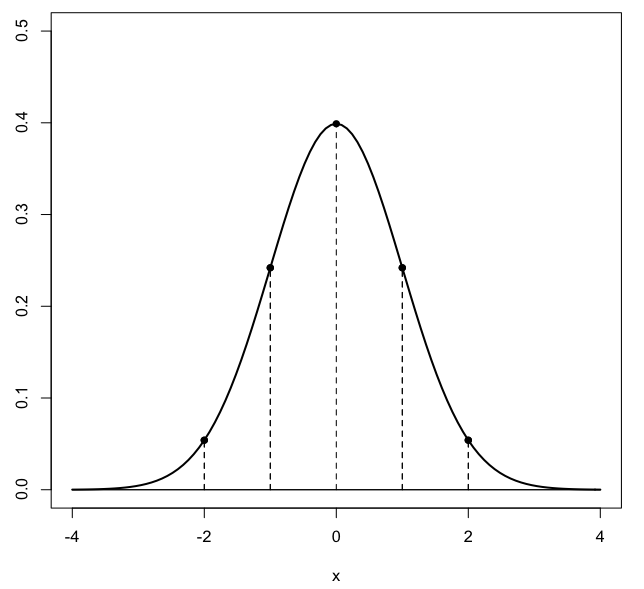
\includegraphics [scale=0.4] {gauss3.png} \end{center}
% \begin{bmatrix} a  &  b \\ c  &  d \end{bmatrix}
% \bigg |_

\large
\noindent
Probably everyone knows the Fibonacci numbers.  Start with 
\[ 1,\ 1,\ 2 \]
The third term is the sum of the previous two.  And the next term is the sum of the previous two 
\[ 1,\ 1,\ 2,\ 3 \]
And so on..
\[ 1,\ 1,\ 2,\ 3,\ 5,\ 8,\ 13,\ 21,\ 34,\ 55,\ 89,\ 144,\ 233 \cdots \]
One interesting thing about the series is that the ratio of successive elements approaches the "golden ratio."
\begin{center} 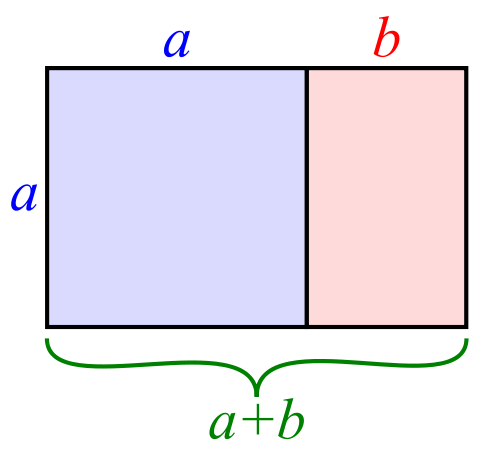
\includegraphics [scale=0.4] {gm.png} \end{center}
In the figure above, if the whole rectangle and the left-hand rectangle have the same proportions, that proportion is the golden mean
\[ \frac{a+b}{a} = \frac{a}{b} =  \phi \]
\[ \phi = \frac{a}{b} = \frac{a+b}{a} = 1 + \frac{b}{a} =  1 + \frac{1}{\phi} \]
so
\[ \phi^2 - \phi - 1 = 0 \]
\[ \phi = \frac{1 \pm \sqrt{5}}{2} = 0.5 \pm 1.118034 \]
These are often called $\phi_1$ and $\phi_2$
\[ \phi_1 = 1.618034 \]
\[ \phi_2 = -0.618034 \]
For right now, I prefer to stick with $\phi$ and $1/\phi$.

Going back to the Fibonacci numbers
\[ 89/55 = 1.6181818  \ \ (> \phi) \]
\[ 144/89 = 1.617976  \ \ (< \phi) \]
\[ 233/144 = 1.618055  \ \ (> \phi) \]
Each successive number is first above and then below $\phi$, and the absolute value of the difference gets smaller with each successive term.

One way of computing successive Fibonacci numbers would be to multiply by $\phi$ and then round to the nearest whole number.  The next one after $233$ is $377$:
\[ 233 \times \phi = 233 \times 1.618034 \]
\[ \ \ = 377.001922 \cong 377 = 144 + 233 \]

But what would be really nice would be to compute the nth Fibonacci number without finding all the ones that come before it.

Binet's formula will do that
\[ F_n = \frac{1}{\sqrt{5}} (\phi^n + (1/\phi)^n) \]

For any $n > 4$ you can ignore the second term ($(1/\phi)^4=0.014$, $(1/\phi)^n \to 0$.
\[ F_n = \frac{\phi^n}{\sqrt{5}} \]
\[ F_{13} = \frac{(1.618034)^{13}}{\sqrt{5}} = 232.999163 \]
Here the formula is exact, the error is in the rounding of the value of $\phi$.  There is some really nice linear algebra related to Fibonacci, but I'll put that in a separate write-up.



\end{document}  